\section{讨论与局限}\label{sec:discussion}

\begin{enumerate}
\item \textbf{SDP 等价的范围与状态。} $10\times10$ Veronese 结果针对的是精确平移消去之后的旋转子问题，它与已发布 $13\times13$ 实现的关系具有已被证明的三部分结构（定理~\ref{thm:thirteen}）。(i) 在完整 20 维理想下，$13\times13$ 松弛\emph{恰好}就是 $10\times10$ 那一个——值相等、秩也相等，由保秩的块 Schur 双射保证——所以一旦理想完备，$10\times10$ 理论确实覆盖了 $13\times13$ 松弛。(ii) 已发布的 24 约束实现只张成 17 维，恰好缺少 $r_1\cdot r_2=r_1\cdot r_3=r_2\cdot r_3=0$，因此一般而言严格更松：$f^\star_{13,\mathrm{up}}\le f^\star_{13,\mathrm{full}}=f^\star_{10,\mathrm{full}}\le f^\star_{\mathrm{QPEP}}$，在对称破缺扰动后有 $8/8$ 个严格间隙（$2.5\times10^{-3}$--$1.4\times10^{-2}$，秩 $\{4,5\}$ 对 6）。(iii) 一个权重为正、真值旋转唯一的 6 点物理 3D--3D 实例以 $1.8207$ 把两者分开，秩为 1 对 4，尽管完整 20D SDP 在该处恰好紧且秩为一。此项已关闭，而不是重新打开：补充材料中“已发布 24 约束松弛与 $10\times10$ 同值”的旧主张才是错误的那个，$10\times10$ 理论不受影响。构造实例的可实现性是另一个问题，仍然开放（第 2 项）。
\item \textbf{Choi--Lam 实例的可实现性。} 构造出的 $M$ 是一个合法的对称代价矩阵，但我们尚未证明它来自真实的 PnP 或矩阵加权对应关系；对\emph{物理}代价矩阵的正测度主张是开放的。在此之前，例~\ref{ex:choilam} 只是关于旋转子问题的陈述，而不是关于 SDPRLayers 生产行为的陈述。第~\ref{sec:results_sdp} 节的 6 点实例\emph{是}物理的，且无需构造目标就分离出了上游实现。
\item \textbf{根枚举。} 前向传播的全局性不会超过求解器本身：漏根、重根与数值消去失败，都会同时破坏“全局”主张与 Laplace 求和。我们把完备性当作假设，并验证残差。计数问题已被测量（$4/4$ 个实例上 40 个复射影根，实根计数 $26/12/12/20$，实局部极小值 $5/2/2/4$）；剩下的是对实际所用枚举器的认证，即多起点牛顿相对同伦在每个实例上的漏根率。逐实例认证的实根计数（带重数的 Sturm/同伦方法）是未来工作。
\item \textbf{Laplace 偏差、折叠与两个折叠定理。} $O(\tau)$ 误差是非一致的。在鞍结（折叠）处模式数发生变化，仅实根的 Laplace 求和甚至不连续。我们对精确平滑后验（第~\ref{sec:laplace} 节）主张光滑性，而对 Laplace 实现只在远离折叠处主张。第~\ref{sec:fold6d} 节测量了两面：在 $\theta=0$ 处 Laplace 映射光滑（其跳变随 FD 斜率 $\approx502$ 线性衰减，而硬映射的跳变保持 $2.86$），但在 $\theta_f\approx1.31\times10^{-3}$ 处存在一个真正的折叠，该处极小值消亡、其权重达到 $0.122$、$\|d\phi\|$ 峰值为 $3529$、位姿映射跳变 $0.31$。更小的 $\tau$ 或更多起点都不能消除该跳变；$\det(H+\tau^{1/3}I)$ 正则化器把导数尖峰降低 24 倍，并把近折叠梯度误差从 $2.9\times10^{-1}$ 降到 $1.2\times10^{-2}$，但只把取值跳变减半（$0.309\to0.107$）。有两个结果解释了原因。

\begin{proposition}[实根代理必然跳变]\label{prop:q5b}
设 $J_\theta$ 在 $\theta_f$ 处经历一个标准的余维 1 折叠（$A_2$）：在它们存在的那一侧（$\theta\to\theta_f^+$），一个次级实极小值 $q_+$ 与邻近的鞍点 $q_-$ 合并为 $q_0$（一个 Hessian 特征值 $\lambda_1(q_+)\to0^+$、横向 Hessian $H_\perp(q_0)\succ0$，并且在别处有一个更深的极小值，满足 $J_0=J_{\theta_f}(q_0)>J_{\rm glob}$），而在另一侧该实极小值消失，于是 $K\to K-1$。那么，任何只对实局部极小值求和、并给合并模式一个正的正则化底权重的代理
\begin{equation}
\tilde w_+^{\rm reg}(\theta_f^+)=\frac{(2\pi\tau)^{3/2}}{\sqrt{\det(H_++\eta(\tau)I_3)}}\,e^{-J_0/\tau},
\label{eq:floorweight}
\end{equation}
在尺度匹配的底 $\eta(\tau)=c_0\tau^{1/3}$ 下，会迫使平滑损失 $\bar\ell_{\rm reg}$ 在 $\theta_f$ 处跳变（其中 $Z_{\rm rest}$ 是其余模式的 Laplace 配分函数）：
\begin{equation}
\begin{split}
&\lim_{\theta\to\theta_f^+}\bar\ell_{\rm reg}-\lim_{\theta\to\theta_f^-}\bar\ell_{\rm reg}\\
&\quad=\frac{\tilde w_+^{\rm reg}(\theta_f^+)}{\tilde w_+^{\rm reg}(\theta_f^+)+Z_{\rm rest}(\theta_f)}\\
&\qquad\times\big(\ell(q_0)-\bar\ell_{\rm rest}(\theta_f)\big)\neq0,
\end{split}
\label{eq:jump}
\end{equation}
并且对 $\eta=c_0\tau^{1/3}$，跳变量为 $\Theta\big(\tau^{1/3}e^{-(J_0-J_{\rm glob})/\tau}\big)$。
\end{proposition}

只有当 $J_0-J_{\rm glob}\gg\tau$ 时它才指数小；当 $J_0-J_{\rm glob}=O(\tau)$ 时它保持 $O(1)$；在任何有限 $\tau$ 下它都非零。这是一个必要性陈述，而不是实现缺陷，也正是 $0.309\to0.107$ 不会趋于零的原因。

\begin{proposition}[复共轭根与 Scorer 延拓]\label{prop:q5c}
40 根作用矩阵求解器把合并对作为复共轭对带过折叠。在正规形
\begin{equation}
J_\theta(u,v)=J_0(\theta)+\tfrac12v^\top H_\perp(\theta)v+\tfrac{c_3(\theta)}{6}u^3-\alpha(\theta)u
\label{eq:normalform}
\end{equation}
中，$c_3>0$、$\alpha(\theta_f)=0$、$\alpha'(\theta_f)>0$（Gromoll--Meyer 分裂）；定义不变量 $J_0=(J(q_+)+J(q_-))/2$ 与 $\zeta(\theta,\tau)=\alpha(\theta)\big(2/c_3(\theta)\big)^{1/3}\tau^{-2/3}$，以及半线 Airy（Scorer）积分
\begin{equation}
\mathcal{S}(\zeta)=\int_0^{+\infty}e^{-s^3/3+\zeta s}\,ds,
\label{eq:scorer}
\end{equation}
它整函数，且 $\mathcal{S}(0)=\Gamma(1/3)/3^{2/3}\approx1.2879$。把两个实根权重换成单个延拓
\begin{equation}
\begin{split}
\tilde w_{\rm fold}(\theta,\tau)={}&\frac{2\pi\tau}{\sqrt{\det H_\perp(\theta)}}\,\tau^{1/3}\Big(\frac{2}{c_3(\theta)}\Big)^{1/3}\\
&\times e^{-J_0(\theta)/\tau}\,\mathcal{S}\big(\zeta(\theta,\tau)\big),
\end{split}
\label{eq:foldweight}
\end{equation}
得到一个在 $\theta_f$ 两侧都是 $C^\infty$ 且取值跳变为零的映射，因为 $(J_0,\alpha,c_3,H_\perp)$ 是特征多项式的对称函数，而 $\mathcal{S}$ 是整函数。对 $\zeta\gg1$，它退化为幸存极小值的普通三维 Laplace 权重 $\tilde w_{\rm fold}=\tilde w_{\rm Lap}(q_+)\big(1+O(\tau/\Delta J_{\rm bar})\big)$；对 $\zeta\ll-1$，它光滑衰减，$\mathcal{S}(\zeta)=|\zeta|^{-1}\big(1+O(|\zeta|^{-3})\big)$。
\end{proposition}

\textbf{该延拓是在不变量层面实现的。} 在 $\theta_f=1.3185\times10^{-3}$ 处的 6D 折叠被双侧跟踪（实极小值/鞍点对与复共轭对），四个不变量 $(J_0,\alpha,c_3,H_\perp)$ 与 $\mathcal{S}(\zeta)$ 在其两侧连续，实测位姿跳变为 $1.21\times10^{-2}$，而标准方法为 $3.04\times10^{-1}$、$\tau^{1/3}$ 方法为 $1.07\times10^{-1}$，即处于光滑映射的导数尺度（$|d\phi|\sim6\times10^2$，跳变/步长为 $6.0\times10^2$ 对 $1.5\times10^4$）。需要注意：把实测不变量等同于正规形只是首阶的（该四次型的四阶系数为 $\approx8.3$），而且这个 6D 折叠很浅（$\Delta J\sim10^{-6}\ll\tau$），因此在折叠\emph{处} Scorer 权重远离其三维 Laplace 极限。主表报告的仍然是仅实根层；它的跳变正是命题~\ref{prop:q5b} 所预言的那个。

\begin{table}[t]
\centering
\caption{6D 折叠处 Scorer 延拓与实根代理的对比（$\theta_f=1.3185\times10^{-3}$、$\tau=0.01$、网格 $\theta_f\pm10^{-4}$、步长 $2\times10^{-5}$）。\emph{跳变}是相邻位姿差的最大值；真正的阶跃在细化下会使\emph{跳变/步长}增长，而光滑映射的\emph{跳变/步长}处于 $|d{\rm pose}|$ 尺度（$\sim6\times10^2$）。}
\label{tab:scorer}
\footnotesize
\setlength{\tabcolsep}{4pt}
\begin{tabular}{@{}l l l l@{}}
\toprule
变体 & 最大跳变 & 跳变 / 步长 & 网格上的 $K$\\
\midrule
标准实根 Laplace & 3.04e-01 & 1.52e+04 & 3--4\\
$\det(H+\tau^{1/3}I)$ 正则化 & 1.07e-01 & 5.34e+03 & 3--4\\
Scorer 延拓 & 1.21e-02 & 6.03e+02 & 4\\
\bottomrule
\end{tabular}
\par\smallskip
\begin{minipage}{\columnwidth}\scriptsize
证据级别：\emph{独立复现（本仓库）}；来源 \path{theory/results/scorer_fold.md}。一维三方校验重现了证明中的 $0.867/0.497/0.3391$，误差 $\le1.6\times10^{-4}$。
\end{minipage}
\end{table}

连续性主张通过网格细化来检验（交错网格，半宽 $10^{-4}$，步长 $d\in\{4\times10^{-5},\ldots,2.5\times10^{-6}\}$）：Scorer 的\emph{跳变/$d$} 在 $d$ 变化 $16\times$ 的范围内保持 $404.3,404.2,404.0,403.7,403.3$（在 $d=2.5\times10^{-6}$ 处没有数值下限），而标准映射的\emph{跳变/$d$} 从 $7.6\times10^{3}$ 增长到 $2.1\times10^{5}$，正则化映射的则从 $2.7\times10^{3}$ 增长到 $4.4\times10^{4}$（一个常数阶跃）。这取代了早先“未做细化检验”的保留意见。因此，折叠邻域落在仅实根 Laplace 层的适用范围之外：要主张连续性，就需要 Scorer 延拓，或对合并对做局部数值积分。

\begin{figure*}[t]
\centering
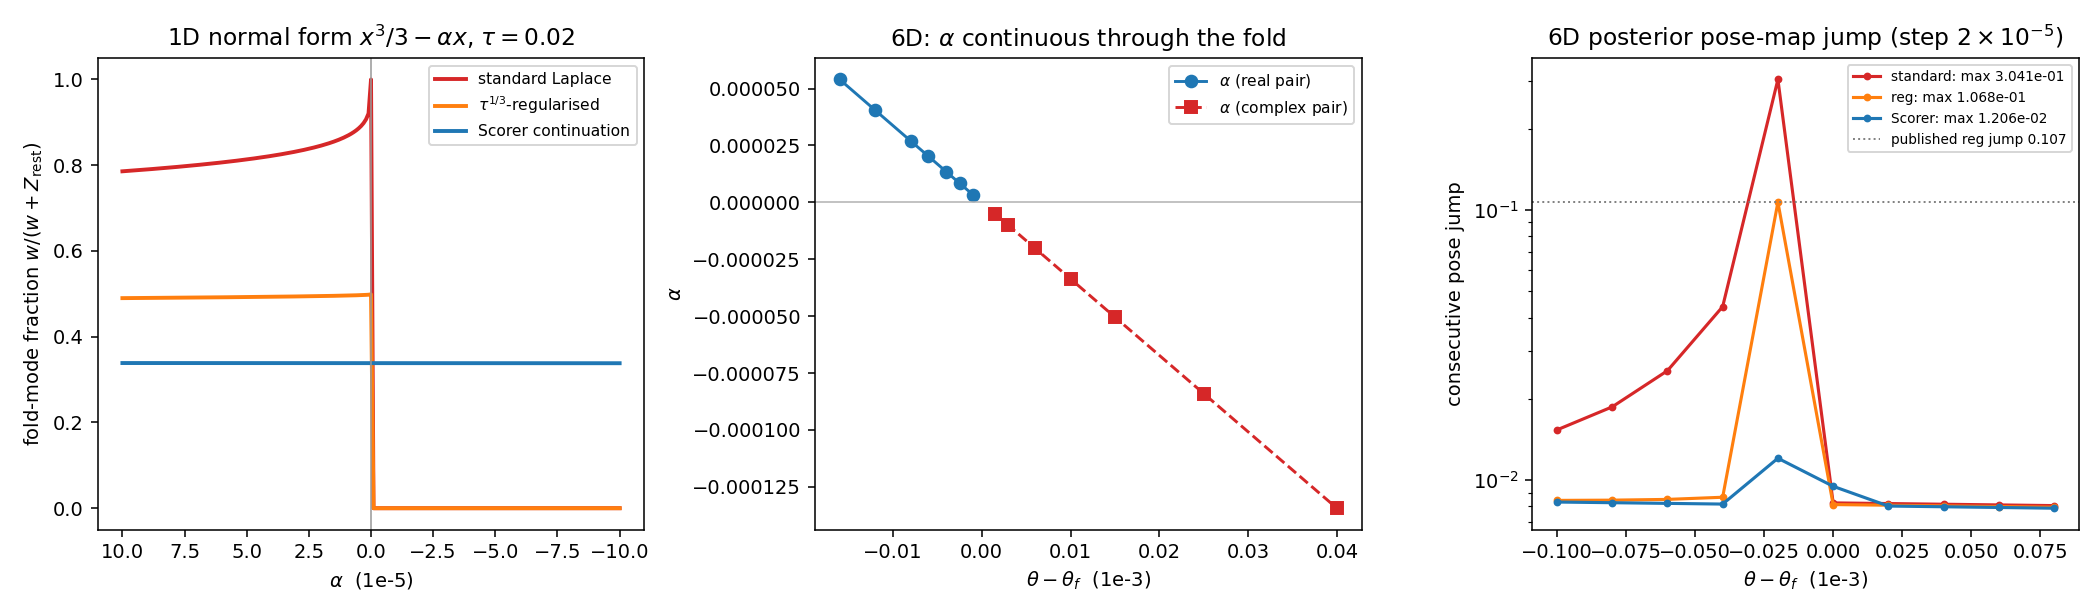
\includegraphics[width=\textwidth]{scorer_fold.png}
\caption{折叠处的 Scorer 延拓。\textbf{左：}一维正规形 $x^3/3-\alpha x$，$\tau=0.02$；折叠模式的权重占比对标准 Laplace 求和而言是不连续的，对 $\tau^{1/3}$ 正则化体积因子从 $0.4959$ 跳到 $0$，而对 Scorer 延拓则是连续的（$0.33838\to0.33834$）。\textbf{中：}$\theta_f=1.3185\times10^{-3}$ 处的 6D 折叠；不变量 $\alpha$ 被穿过折叠跟踪，在实根对/复根对切换处连续。\textbf{右：}最大相邻后验位姿跳变相对 $\theta-\theta_f$：标准映射尖峰到 $3.04\times10^{-1}$，正则化映射到 $1.07\times10^{-1}$，而 Scorer 延拓的峰值为 $1.21\times10^{-2}$，处于光滑映射的导数尺度。}
\label{fig:scorer}
\end{figure*}

\item \textbf{对称物体：一个正结果及其精度代价。} 新的真实数据构造在 15/15 个 LINEMOD \texttt{eggbox}/\texttt{glue} 帧上产生两个真正的模式，而实测结果并不是精度胜利：硬 argmin 在近平局处是准确的（中位数 $2.06^\circ$、ADD-S $3.7$ mm，处于经典前向求解器的水平），而 Laplace 均值被拉向翻转（中位数 $44.24^\circ$、ADD-S $13.9$ mm；配对偏差 $+36.9^\circ$）。这就是该层所做的精度/光滑性取舍，而且对称物体上的行为现在是被测量过的，而不是未被测试的。
\item \textbf{三阶导数。} $\nabla_\theta\log\det H_k$ 需要 $J$ 的三阶 $q$ 导数以及 $q^{(k)}$ 的隐式导数；对四次型而言可以处理，但要正确实现并不简单。它是“$3\times3$ 反向传播”这一口号与完整 Laplace KL 之间的主要差距。
\item \textbf{温度。} $\tau$ 是一个依赖代价尺度的超参数。没有尺度归一化时它不可辨识；有了尺度归一化，$\tau$ 就可以学习。$\tau\to0$ 极限只对后验均值/argmin 恢复确定性梯度，对原始 KL 损失则不然。
\item \textbf{没有不等式约束，也没有外点鲁棒性。} 这些被委托给伴随工作线：该层假设 $G\succ0$ 与固定的加权 Gram 矩阵，不处理非穿透、手性不等式或严重外点。
\item \textbf{GPU 批处理。} 代数根枚举是工程瓶颈；一个批量的 $40\times40$ 复特征值求解器看起来可行，但尚未基准测试。
\end{enumerate}
